\documentclass[11pt]{article}
\usepackage{anysize}
\marginsize{1.2cm}{1.4cm}{.4cm}{1cm}

\usepackage[normalem]{ulem}
\usepackage{amsfonts}
\usepackage{amsmath}
\usepackage[shortlabels]{enumitem}
\usepackage{graphicx}
\usepackage{listings}
\lstset{
  basicstyle=\ttfamily,
  mathescape
}

\setlength{\parindent}{0pt}

\newcommand{\by}{\mathbf{y}}
\newcommand{\bY}{\mathbf{Y}}
\newcommand{\bX}{\mathbf{X}}
\newcommand{\btheta}{\mathbf{\theta}}
\newcommand{\bI}{\mathbf{I}}
\newcommand{\bA}{\mathbf{A}}
\newcommand{\bB}{\mathbf{B}}
\newcommand{\bW}{\mathbf{W}}

\newcommand{\thh}{\hat{\theta}}
\newcommand{\yh}{\hat{y}}
\newcommand{\sgn}{\text{ sign}}
\DeclareMathOperator*{\argmin}{arg\,min}
\newcommand{\pcd}{\text{PATHWISE\_CD}}

\begin{document}

Ian Dardik \\
Heeru Ahuja \\
CS6140 \\
Exploring Regularization Techniques for Small Data Sets

\section{Introduction}
In this paper we focus on regularization techniques that improve linear regression modeling on small data sets.  Ordinary Least Squares (OLS) is a popular solution for the weights of a linear model, however the method becomes numerically unstable as the number of samples decrease, and has no solution when the number of parameters exceed the sample size.  Statistical regularization techniques stabilize our solution and reduce the variance which becomes increasingly important as the number of samples in our data set shrink.  Unforunatley, statistical regularization introduces bias into our model so we must choose an appropriate balance.  The models we consider in this paper control the degree of regularization through one or two tuning parameters that are completely suppressed at zero, and have more influence on the solution as they increase towards infinity.  We can estimate the ideal tuning parameter values by using cross-validation to estimate the MSE for a small universe of tuning parameters, and select the parameters that minimize MSE.  Each regularization technique that we consider is formulated as an optimization problem that minimizes an objective function $J$ of the form:
	$$\thh = \argmin\limits_\theta J(\theta) =\argmin\limits_\theta \sum\limits_{i=1}^N L(\theta) + \sum\limits_{i=1}^P R(\theta,\lambda)$$

Where $L(\theta)$ is the loss function and $R(\theta,\lambda)$ is the regularization rule that depends on the tuning parameter $\lambda$, and sometimes an additional tuning parameter $\alpha$.  We often refer to the regularization rule as the \textit{penalty}.  We only consider squared loss in this paper, i.e. $L(\theta)= (Y_i - X_i'\theta)^2$, however we consider and discuss several options for choice of the regularization rule.  The regularization techniques that we consider are:
\begin{itemize}
	\item L1 penalty (LASSO)
	\item L2 penalty (Ridge)
	\item L$\frac{1}{2}$
	\item Elastic Net
	\item L2 with Custom Soft-Thresholding
\end{itemize}

Many of the regularization techniques we discuss do not have a closed analytical solution, so we will consider two algorithms for numerically arriving at a solution: Batch Gradient Descent and Pathwise Coordinate Descent.  The following sections detail how to use each regularization rule with each algorithm.  \\

For the remainder of this paper we assume that all data $X$ and responses $Y$ are standardized.  

\section{Gradient Descent}
Gradient Descent algorithms work by moving in the direction that the gradient of $\theta$ points, with distance scaled by a learning rate parameter $\alpha$.  The algorithm continuously updates it value for the parameter vector $\theta$ until convergence.  Gradients point towards local optima, so we clearly need to use convex objective functions to arrive at a gobally optimal solution in Gradient Descent.  Fortunately, computing the gradient of objective functions listed above is straightforward which makes Gradient Descent fairly simple to implement.  Notice that Gradient Descent works by computing the gradient; it does not itself solve an optimization problem per se; since the algorithm is only dependent on the gradient of the objective function, we can parameterize it based on the gradient.  Therefore we end up with a core algorithm the form: $\text{gradient\_descent}(\nabla\theta, X, Y)$

\section{Pathwise Coordinate Descent}
While Gradient Descent operates on the entire parameter vector at once, Pathwise Coordinate Descent (PCD) concentrates on each parameter individually.  Pathwise Coordinate Descent considers each parameter $\theta_j$ as its own optimization problem\cite{ht}:
	$$\thh_j = \argmin\limits_{\theta_j} J(\theta)$$

In each iteration of the PCD algorithm, we update each $\theta_j$ to be the solution to the individual optimization problem.  

\subsection{Parameterizing the PCD Algorithm}
Pathwise Coordinate Descent is parameterized by the objective function $J$ that it solves for each $\theta_j$.  However, for the universe of objective functions we consider in this paper, we can parameterize the PCD algorithm by just two nonnegative parameters we call $A$ and $B$.  For each objective function we consider below, we will show that the solution to optimizing each $\theta_j$ takes the form:
	$$\theta_j = S\left(\sum\limits_{i=1}^N X_{ij}(Y_i - \sum\limits_{k \ne j}^p X_{ik}\theta_k), B\right)/A$$

Where we define\cite{ht} $S(t,B) = \sgn(t)(|t|-B)_+$, and $()_+$ is the soft-thresholding operator.  It follows that each algorithm reduces to the following parameterized form $\pcd(A, B)$.  In the following sections we will show how each of the objective functions we consider fit into this parameterization.  

\subsection{LASSO}
LASSO uses the L1 norm for a penalty:
	$$\thh_j = \argmin\limits_{\theta_j} \frac{1}{2} \sum\limits_{i=1}^N \left(Y_i - \sum\limits_{k=1}^px_{ik}\theta_k \right)^2 + \lambda \sum\limits_{k=1}^p|\theta_k|$$

Where $\lambda \geq 0$ is a tuning parameter.  Let $J$ be the objective function we want to optimize above.  We can solve for $\theta_j$ by finding the stationary points of $J$:
\begin{equation}\begin{split}
	\frac{\partial J}{\partial \theta_j}
		& = -\sum\limits_{i=1}^N X_{ij}(Y_i - X_{ij}\theta_j - \sum\limits_{k \ne j}^p X_{ik}\theta_k) + \lambda \sgn(\theta_j) \\
		& = -\sum\limits_{i=1}^N X_{ij}(Y_i - \sum\limits_{k \ne j}^p X_{ik}\theta_k) + \sum\limits_{i=1}^NX_{ij}^2\theta_j + \lambda \sgn(\theta_j) \\
		& = -\sum\limits_{i=1}^N X_{ij}(Y_i - \sum\limits_{k \ne j}^p X_{ik}\theta_k) +(N-1)\theta_j + \lambda \sgn(\theta_j) \\
\end{split}\end{equation}

The last step follows from the fact that our data is standardized, and thus $\sum\limits_{i=1}^NX_{ij}^2 = N-1$.  \\

Set $\frac{\partial J}{\partial \theta_j}=0$ and, for convenience, let $Q = \sum\limits_{i=1}^N X_{ij}(Y_i - \sum\limits_{k \ne j}^p X_{ik}\theta_k)$ and and we get:
	$$(N-1)\theta_j + \lambda\sgn(\theta_j) = Q$$

To solve for $\theta_j$ notice that when $\theta_j \geq 0$, $\theta_j=\frac{Q-\lambda}{N-1}$ so $Q \geq \lambda$.  However when $\theta_j \leq 0$, $\theta_j=\frac{Q+\lambda}{N-1}$ so $Q \leq -\lambda$.  Notice the following two properties: \\
	\hspace*{1cm} (1) $|Q| \geq \lambda$ \\
	\hspace*{1cm} (2) $\theta_j \geq 0$ iff $Q \geq 0$ and $\theta_j \leq 0$ iff $Q \leq 0$ \\

Therefore, we can write the solution for $\theta_j$ as:
	$$\theta_j = \frac{\sgn(Q)(|Q|-\lambda)_+}{N-1}$$

Where the soft-thresholding operator guarantees property (1), while multiplying by $\sgn(Q)$ makes use of (and guarantees) property (2).  Recall from Section 2 that $S(t,B) = \sgn(t)(|t|-B)_+$, then our final solution is:
	$$\theta_j = S\left(\sum\limits_{i=1}^N X_{ij}(Y_i - \sum\limits_{k \ne j}^p X_{ik}\theta_k), \lambda\right)/(N-1)$$

Notice this yields a solution nearly identical to Elements of Statistical Learning\cite{ht}; the difference is that we divide by $N-1$ and we believe this is likely a typo in the book.  \\

Notice that the soft-thresholding parameter is $\lambda$; this explains why larger $\lambda$ values causes LASSO to drive parameter values to zero.  It is now clear that LASSO performs subset selection due to the choice of regularization penalty \textit{and} algorithm.  \\

Finally, it is clear that the parameterization for LASSO is $\pcd(N-1,\lambda)$.  


\subsection{Elastic Net}
The Elastic Net uses the tuning parameter $\alpha \in [0,1]$ to compromise between Ridge and Lasso penalization.  Ridge penalizes the L2 norm, so Elastic Net solves the following optimization problem:
	$$\thh_j = \argmin\limits_{\theta_j} \frac{1}{2} \sum\limits_{i=1}^N \left(Y_i - \sum\limits_{k=1}^px_{ik}\theta_k \right)^2 + \lambda \sum\limits_{k=1}^p \left(\alpha\theta_k^2 + (1-\alpha)|\theta_k| \right)$$

This math is very similar to LASSO above so we have left the details to the appendix.  Our final solution is:
	$$\theta_j = S\left(\sum\limits_{i=1}^N X_{ij}(Y_i - \sum\limits_{k \ne j}^p X_{ik}\theta_k), B\right)/A$$

Where $A=(N-1)+2\lambda\alpha$, and $B=\lambda(1-\alpha)$.  This equation is already in our desired form, and hence the parameterization is $\pcd(N-1+2\lambda\alpha,\lambda(1-\alpha))$.  

\subsection{Ridge}
Ridge Regularization has a closed form analytical solution so it does not require an algorithm.  Nevertheless, we will discuss Ridge in the context of PCD to realize why the L2 penalty does not perform subset selection while the L1 does.  We can simply use our solution for the Elastic Net with $\alpha=1$ for the Ridge solution.  This implies that $A=(N-1)+2\lambda$ and $B=0$, yielding:
	$$\theta_j = S\left(\sum\limits_{i=1}^N X_{ij}(Y_i - \sum\limits_{k \ne j}^p X_{ik}\theta_k), 0\right)/(N-1+2\lambda)$$

With parameterization $\pcd(N-1+2\lambda,0)$.  Notice that the soft-thresholding parameter is zero; this implies that \textit{no} soft-thresholding will be applied for Ridge, regardless of the parameter $\lambda$.  This explains why Ridge tends to shrink parameter values but doesn't drive them towards zero.  

\subsection{Custom Shrinkage Methods}
We have found above that LASSO uses $\lambda$ exclusively for linear shrinkage and soft-thresholding, while Ridge uses $\lambda$ exclusively for inverse shrinkage.  We propose three ``custom" ideas for changing and combining the shrinkage types in the context of PCD:

\subsubsection{Ridge with Soft-Thresholding}
This customization, inspired by Nearest Shrunken Centroids, applies soft-thresholding to the Ridge solution.  This yields the parameterization $\pcd(N-1 + 2\lambda, \gamma)$, where the tuning parameter $\gamma$ governs the degree of soft-thresholding.  We found that cross-validation does not perform well for selecting a good $\lambda, \gamma$ pair so we instead consider the case where $\gamma=\lambda$, yielding $\pcd(N-1 + 2\lambda, \lambda)$.  

\subsubsection{Ridge with Quadratic Soft-Thresholding}
This idea is similar to the previous, except we vary the soft-thresholding quadratically with respect to the tuning parameter $\lambda$: $\pcd(N-1 + 2\lambda, \lambda^2)$.  

\subsubsection{Ridge with Exponential Soft-Thresholding}
This idea is similar to the previous two, except we vary the soft-thresholding exponentially with respect to the tuning parameter $\lambda$: $\pcd(N-1 + 2\lambda, e^\lambda-1)$.  

\section{Results}
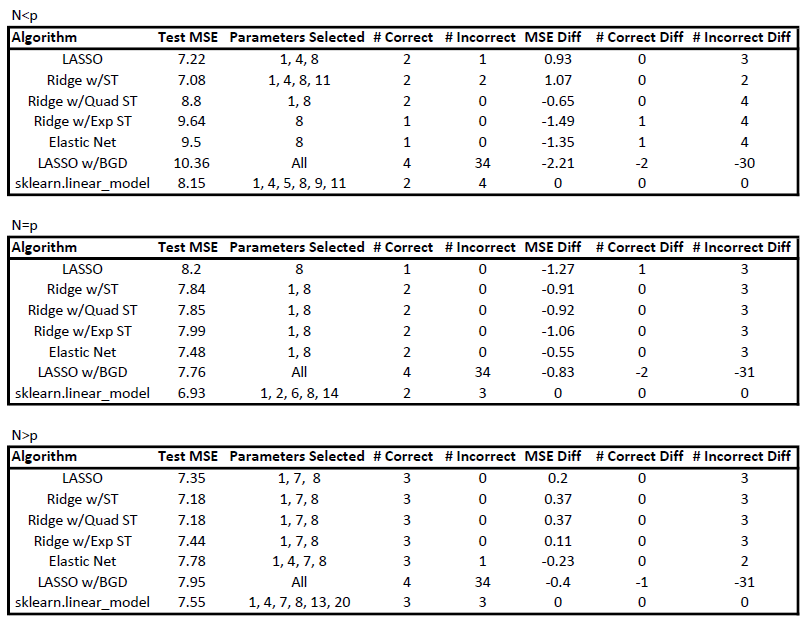
\includegraphics[scale=0.6]{ortho.PNG} \\
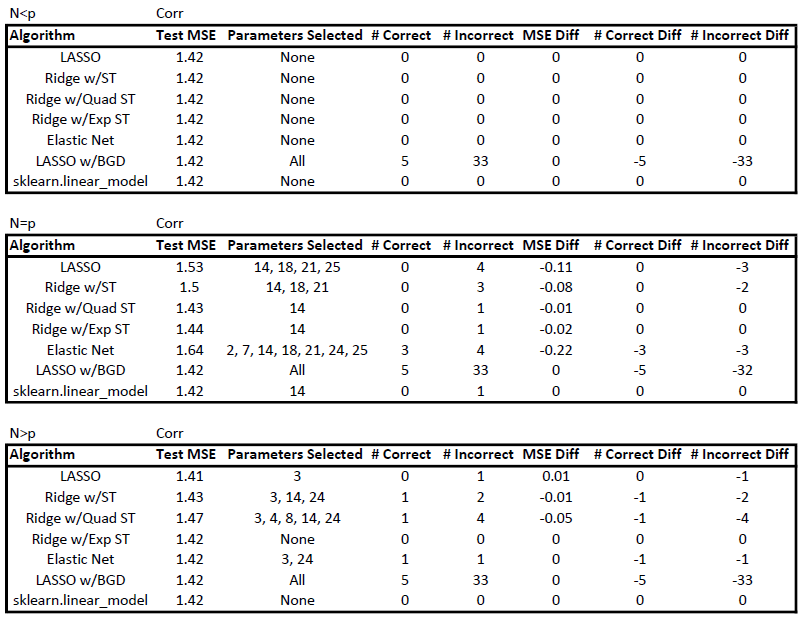
\includegraphics[scale=0.6]{corr.PNG}

\begin{thebibliography}{9}
\bibitem{ht} 
Trevor Hastie, Robert Tibshirani, and Jerome Friedman,
The Elements of Statistical Learning 2nd Edition
\end{thebibliography}

\end{document}














